
%%%  یک نمونه پروپوزال کارشناسی ارشد، نسخه 0.4
%%%  وحید دامن‌افشان، دانشگاه تبریز،       http://www.damanafshan.ir
%%%   آپدیت شده در تیرماه ۹۱
%توضیحات مربوط به هر بسته یا دستور را می‌توانید در خط بالای آن ببینید.

\documentclass[12pt,a4paper]{article}
%در ورژن جدید زی‌پرشین برای تایپ متن‌های ریاضی، این سه بسته، حتماً باید فراخوانی شود
\usepackage{amsthm,amssymb,amsmath}

%دستوری برای وارد کردن واژه‌نامه انگلیسی به فارسی
\newcommand\persiangloss[2]{#1\dotfill\lr{#2}\\}
%بسته‌ای برای تنطیم حاشیه‌های بالا، پایین، چپ و راست صفحه
%\usepackage[top=30mm, bottom=30mm, left=30mm, right=30mm]{geometry}
%بسته‌ای برای نمایش تصاویر قرار داده شده در متن
\usepackage{graphicx}
% بسته‌ و دستوراتی برای ایجاد لینک‌های رنگی با امکان جهش
\usepackage[pagebackref=false,colorlinks,linkcolor=blue,citecolor=magenta]{hyperref}
% چنانچه قصد پرینت گرفتن نوشته خود را دارید، خط بالا را غیرفعال و  از دستور زیر استفاده کنید چون در صورت استفاده از دستور زیر‌‌، 
% لینک‌ها به رنگ سیاه ظاهر خواهند شد و برای پرینت گرفتن، مناسب‌تر خواهد بود.
%\usepackage[pagebackref=false]{hyperref}
%بسته‌ای برای ظاهر شدن «مراجع»  در فهرست مطالب
\usepackage{tocbibind}
%فراخوانی بسته زی‌پرشین و دستورات مربوط به نوع فونت‌ها
\usepackage{xepersian}
%تغییرات نخ
\usepackage[bottom]{footmisc}
\usepackage{indentfirst}


\settextfont{B Nazanin}
% وارد کردن دستور بالا الزامی نیست؛ چون در صورت وارد نکردن آن، فونت پیش‌فرض به صورت خودکار، فراخوانی می‌شود.
% چنانچه می‌خواهید که اعداد داخل فرمول‌ها، فارسی باشد، دستور زیر را فعال کنید
%\setdigitfont{Times New Roman}


%%%%%%%%%%%%%%%%%%%%%%%%%%%%%%%%%%%%%%%%%%%%%%%%%%%
% تعریف قلم‌های فارسی و انگلیسی برای استفاده در بعضی از قسمت‌های متن
\defpersianfont\titr[Scale=1]{B Titr}
\defpersianfont\nastaliq[Scale=1.5]{IranNastaliq}
\defpersianfont\traffic[Scale=1]{B Traffic}
\defpersianfont\yekan[Scale=1]{B Yekan}
\DefaultMathsDigits
%اگر فونت‌های بالا را ندارید، دو خط بالا را غیر فعال و دو خط زیر را فعال کنید
%\defpersianfont\traffic[Scale=1]{XB Roya}
%\defpersianfont\yekan[Scale=1]{XB Kayhan}
%%%%%%%%%%%%%%%%%%%%%%%%%%%%%%%%%%%%%%%%%%%%%%%%%%%
% تعریف و نحوه ظاهر شدن قضایا، لم‌ها، تعریف‌ها و ...
\theoremstyle{definition}
\newtheorem{definition}{تعریف}[section]
\theoremstyle{theorem}
\newtheorem{theorem}[definition]{قضیه}
\newtheorem{lemma}[definition]{لم}
\newtheorem{proposition}[definition]{گزاره}
\newtheorem{corollary}[definition]{نتیجه}
\newtheorem{remark}[definition]{ملاحظه}
\theoremstyle{definition}
\newtheorem{example}[definition]{مثال}
%%%%%%%%%%%%%%%%%%%%%%%%%%%%%%%%%%%%%%%%%%%%%%%%%%%
\begin{document}
% دستوری جهت حذف کردن شماره صفحه و سربرگ، در صورت وجود (فقط در صفحه جاری)
\thispagestyle{empty}
\vspace*{-28mm}
% نحوه درج کردن لوگوی دانشگاه
\centerline{
\includegraphics[height=5cm]{logo.png}}
\begin{center}
%دستوری برای کم کردن فاصله بین لوگو و خط پایین آن
\vspace{-2mm}
{\large \titr
گروه مستقل مهندسی رباتیک
%دستوری برای تعیین فاصله بین دو خط
\\[2.1cm]
}

{\Large \titr
تمرین سوم درس بینایی ماشین
\\[2cm]
استاد درس:
\\[.5cm]
دکتر صفابخش
\\[1.5cm]
\large 
تدریس‌یار: 
\\[0.5cm]
مهندس مجد
\\[1.5cm]
نام دانشجو:
\\[.5cm]
نوید خزاعی
\\[.5cm]
۹۲۱۳۵۰۰۸
\\[1.5cm]
}
%دستوری برای تعیین فاصله بین خطوط (نه دو خط) و تا وقتی که مقدار آن تغییر نکند، فاصله بین خطوط، همین مقدار است.
\baselineskip=1cm

{\large
اردیبهشت ۱۳۹۲
}
\end{center}
%دستوری برای رفتن به صفحه جدید
\newpage
\baselineskip=1cm
%دستوری برای ظاهر شدن فهرست مطالب
\tableofcontents

\baselineskip=.75cm
\newpage 
\section{بخش اول}
%\cite{alvarez}
\subsection{{\lr {K-means‬‬} و ویژگی‌ها
}
}



\textbf{پرسش:}
الف) در این تمرین با استفاده از روش \lr{k} میانگین می‌خواهیم تصاویر شماره‌ی ۷، ۸ و ۹ قطعه‌بندی شود. در این تصاویر چه ویژگی‌هایی را مناسب قطعه‌بندی می‌بینید؟ در صورتی که برای محاسبه‌ی ویژگی‌ها از توابع خاص یا کدی از اینترنت استفاده می‌کنید توضیح دهید.

\textbf{پاسخ:}
در تصویر شماره‌ی ۷، رنگ ویژگی مناسبی است. به این ترتیب که مقادیر \lr{R}، \lr{G} و \lr{B} را به عنوان ویژگی در نظر گرفتیم. محاسبه‌ی این ویژگی بسیار ساده‌است و از خود مقادیر پیکسل‌ها استفاده کردیم. تنها کافی‌است با دستور \lr{img.reshape(rows*cols,3)} تصویر مورد نظر را به شکل برداری سه ستونی درآوریم که در هر سطر، هر پیکسل و در هر ستون، مقادیر ویژگی‌ها قرار داشته‌باشند تا بتوانیم آن را به تابع \lr{kmeans} دهیم که شرح آن در پاسخ سوال بعد آورده شده‌است. برای بهتر شدن نتایج از \lr{medianBlur()} استفاده‌‌نمودیم تا مقادیر رنگ نواحی متفاوت کوچک، با حساب کردن میانه، به مقادیر رنگ نواحی همسایه‌ی خود، نزدیک‌تر شود. دقت کنید که این فیلتر باید با هسته‌ی کوچک و چندین بار اعمال شود تا جزییات به اندازه‌ی کافی از بین برود و از طرفی نواحی رنگی تا حد قابل قبولی مرزهای خود را حفظ کنند. مقادیر اندازه‌ی هسته و تعداد دفعات تکرار فیلتر توسط رابط کاربری قابل تنظیم است تا نتایج بیشتری را ببینید. نتایج را در بخش بعد خواهید دید.
برای دو تصویر دیگر، باید از یک ویژگی که بافت را توصیف کند استفاده کنیم. طبق پژوهش‌های به‌عمل آمده، فیلترهای \lr{Gabor} برای این امر مناسب هستند. به این ترتیب که می‌توان مقادیر واریانس و میانگین حاصل از اعمال هر فیلتر را، به عنوان ویژگی در نظر گرفت. این عمل باید بر روی نواحی مختلف تصویر اعمال شود و از یک پنجره‌ی لغزان برای این کار استفاده‌شود تا ویژگی‌های بافت برای نواحی کوچک استخراج شود. سپس نماینده‌ی هر کدام از این نواحی را، با ویژگی‌های استخراج‌شده‌اش، به الگوریتم \lr{kmeans} دهیم تا دسته‌بندی بافت‌ها صورت گیرد و نتیجه‌ی نهایی‌ را به تصویر اولیه، نگاشت کنیم. متاسفانه به دلیل پیچیدگی پیاده‌سازی این قسمت با زبان \lr{C++} موفق به انجام آن نشدیم.
\\

\subsection{استفاده از \lr{K-means}}
\textbf{پرسش: }
با استفاده از روش \lr{K} میانگین تصویر را قطعه‌بندی کرده و نتایج را نمایش دهید. چه پارامترهایی در این روش وجود دارد و مقدار آن را چگونه تعیین کردید؟

\textbf{پاسخ: } 
پارامتر‌های این روش به ترتیب در زیر آمده‌اند:

\begin{itemize}
\renewcommand{\labelitemi}{$\bullet$}
\item \lr{\textbf{samples}}: نمونه‌های ورودی هستند. به ازای هر نمونه، یک سطر آورده می‌شود و در آن سطر، هر ستون، مقدار یک ویژگی را مشخص می‌کند. برای تصویر شماره‌ی ۷، همان‌گونه که در پاسخ سوال قبل اشاره نمودیم، از تابع عضو کلاس ماتریس به نام \lr{reshape} برای تولید این ماتریس استفاده نمودیم.
\item \lr{\textbf{K}}: تعداد دسته‌های مطلوب. برای تصویر شماره‌ی ۷ این مقدار را برابر ۴ قرار دادیم تا رنگ‌های قرمز، سفید، زرد و قهوه‌ای/سیاه پس‌زمنیه را تفکیک کنیم. همچنین برای دیدن نتایج بیشتر، این مقدار توسط رابط کاربری قابل تعیین است.
\item \lr{\textbf{labels}}: برچسب‌های نهایی که به تعداد نمونه‌ها خواهد بود و مقدار آن، برای هر اندیس، دسته‌ی محاسبه‌شده برای نمونه‌ی متناظر آن اندیس را بیان می‌کند. 
در صورتی که مایل باشیم در اجرای اول، دسته‌های نمونه‌ها را به طور دستی مشخص کنیم، این آرایه را مقداردهی می‌کنیم. در این اجرا، آرایه‌ای ساخته و بدون مقدار دهی به تابع دادیم.
\item \lr{\textbf{criteria}}: شرط خاتمه‌است. برای ایجاد شرط مطلوب، از کلاس 
\lr{TermCriteria}
استفاده کردیم و با \lr{OR} نمودن فلگ‌های شرط تکرار محدود و شرط خطای ابسیلون، با مقدار تکرار ۱۰۰۰ و ابسیلون ۱ که به صورت تجربی به‌دست آوردیم، آن را مشخص نمودیم. 
\item \lr{\textbf{attempts}}: تعداد دفعات اجرای الگوریتم با مقادیر اولیه‌ی متفاوت. این مقدار توسط رابط کاربری قابل تعیین می‌باشد. مقدار پیش‌فرض آن را به صورت تجربی برابر با ۵ قرار دادیم.
\item \lr{\textbf{flags}}: پرچم‌های مورد نیاز. در این‌جا مشخص‌کننده‌ی روش مقدار دهی اولیه‌ی نقاط نماینده‌ی دسته‌ها می‌باشد که آن‌ را برای استفاده از روش مقداردهی تصادفی، تنظیم نمودیم.
\item \lr{\textbf{centers}}: آرایه‌ی نقاط نماینده‌ی هر دسته‌ می‌باشد که به طول \lr{K} است و تعداد ستون‌های آن، برابر با تعداد ویژگی‌هاست که در هر سطر، مقادیر یافت‌شده‌ برای نماینده‌ی آن دسته را در خود دارد.
\end{itemize}

نتیجه برای هسته‌ی میانه به اندازه‌ی ۹ و تعداد تکرار ۲۵ فیلتر میانه:

\vspace{0.2cm}
\begin{center}
\vspace{5mm}
\begin{tabular}{@{}cc@{}}
\frame{
\includegraphics[height=40mm]{7-blured9-25.png}} &
\frame{
\includegraphics[height=40mm]{7-final9-25.png}} \\ 
\small \textbf{دسته‌های یافت‌شده} & \small \textbf{پس از لبه‌یابی}
\end{tabular}
\vspace{0.5cm}
\end{center} 

نتیجه برای هسته‌ی میانه به اندازه‌ی ۲۱ و تعداد تکرار ۳۰ فیلتر میانه:

\vspace{0.2cm}
\begin{center}
\vspace{5mm}
\begin{tabular}{@{}cc@{}}
\frame{
\includegraphics[height=40mm]{7-blured21-30.png}} &
\frame{
\includegraphics[height=40mm]{7-final21-30.png}} \\ 
\small \textbf{دسته‌های یافت‌شده} & \small \textbf{پس از لبه‌یابی}
\end{tabular}
\vspace{0.5cm}
\end{center} 

\subsection{تغییر تعداد خوشه‌ها}

\textbf{پرسش: }
تعداد خوشه‌ها را از ۲ تا ۱۵ خوشه تغییر داده و نتایج حاصل را تحلیل کنید. تصاویر ۱-۷، ۱-۸ و ۱-۹ به ترتیب نتایج قطعه‌بندی روی تصاویر ۷، ۸ و ۹ را نشان می‌دهد. اختلاف نتایج شما با این نتایج چند درصد است؟

\textbf{پاسخ: } 
نتایج برای هسته‌ی ۹ و تکرار ۳۰ در زیر آمده‌است. تعداد خوشه‌ها مشخص شده‌است.


\vspace{0.2cm}
\begin{center}
\vspace{5mm}
\begin{tabular}{@{}cc@{}}
\frame{
\includegraphics[height=40mm]{7-blured9-3015.png}} &
\frame{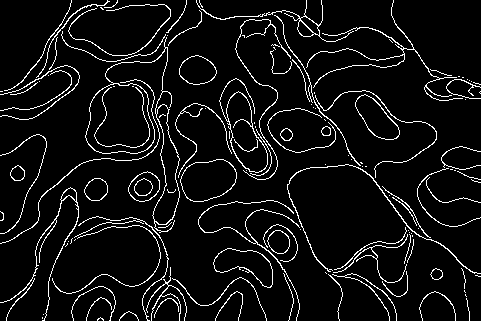
\includegraphics[height=40mm]{7-final9-3015.png}} \\ 
\small \textbf{ ۱۵ دسته‌ یافت‌شده} & \small \textbf{پس از لبه‌یابی}
\end{tabular}
\vspace{0.5cm}
\end{center} 


\vspace{0.2cm}
\begin{center}
\vspace{5mm}
\begin{tabular}{@{}cc@{}}
\frame{
\includegraphics[height=40mm]{7-blured9-3012.png}} &
\frame{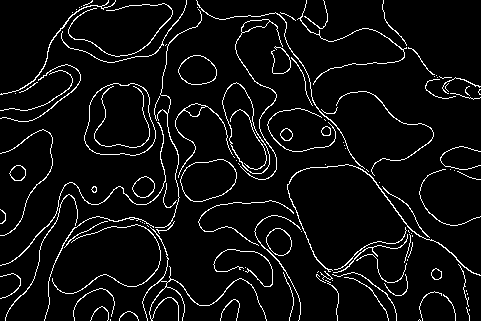
\includegraphics[height=40mm]{7-final9-3012.png}} \\ 
\small \textbf{دسته‌های یافت‌شده ۱۲} & \small \textbf{پس از لبه‌یابی}
\end{tabular}
\vspace{0.5cm}
\end{center} 


\vspace{0.2cm}
\begin{center}
\vspace{5mm}
\begin{tabular}{@{}cc@{}}
\frame{
\includegraphics[height=40mm]{7-blured9-309.png}} &
\frame{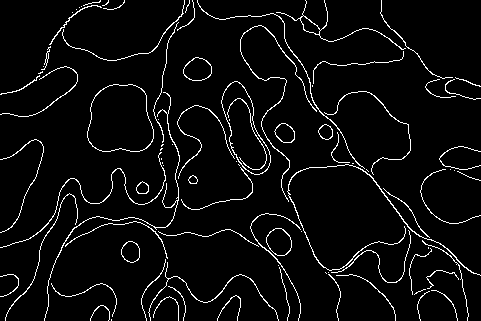
\includegraphics[height=40mm]{7-final9-309.png}} \\ 
\small \textbf{ ۹ دسته‌های یافت‌شده} & \small \textbf{پس از لبه‌یابی}
\end{tabular}
\vspace{0.5cm}
\end{center} 


\vspace{0.2cm}
\begin{center}
\vspace{5mm}
\begin{tabular}{@{}cc@{}}
\frame{
\includegraphics[height=40mm]{7-blured9-304.png}} &
\frame{
\includegraphics[height=40mm]{7-final9-304.png}} \\ 
\small \textbf{دسته‌های یافت‌شده ۴} & \small \textbf{پس از لبه‌یابی}
\end{tabular}
\vspace{0.5cm}
\end{center} 

یعنی با خوشه‌های بیشر، جزییات بیشتری در تصویر نهایی قطعه‌بندی‌شده دیده می‌شود و به خاطر سخت‌گیری در تعیین مرز خوشه‌هاست. 
%دستوری برای به حالت عادی درآمدن اندازه فونت‌ها 


\small
%ایجاد «مراجع»

\end{document} 
